\documentclass{article}
\usepackage[spanish]{babel}
\usepackage[utf8]{inputenc}
\usepackage{float}
\usepackage{hyperref}
\usepackage{cite}
\usepackage{graphicx}
\usepackage{subfigure}
\usepackage{booktabs}
\newcommand{\hal}{$H\alpha$}

\begin{document}
\title{Estudio de la curva de rotación y la masa no bariónica de la galaxia UGC11916}
\author{Iñigo Pérez Mérové-Pierre}
\date{20 de octubre de 2018}
\maketitle

\begin{abstract}
\href{url}{$https://github.com/iperezmerove/proyecto_final$}\\En este trabajo vamos a realizar un estudio de la galaxia con anillo polar UGC1196 a partir de los datos obtenidos de observaciones realizadas con la técnica de espectroscopia de campo integral. Las galaxias con anillo polar, debido a su peculiar morfología y a su origen y evolución, son objetos que nos pueden proporcionar gran información sobre las interacciones galácticas y sobre la naturaleza y distribución de la materia oscura en las galaxias. En primer lugar, realizaremos un análisis morfológico en el continuo de la galaxia, analizando la intensidad del espectro en su zona central. Mediante el estudio del gas ionizado (HII) a través de la línea de \hal, analizando sus mapas de velocidad, la curva de rotación y comparando con las velocidades y curvas de rotación estelares, podemos detectar la presencia de sistemas cinemáticos diferenciados que nos permitan inferir la presencia de anillos polares en estas galaxias. Estudiaremos la relación entre la masa luminosa ($M_{L}$), esto es, la masa total de la galaxia en función de su luminosidad, y la masa dinámica ($M_{D}$), la masa estimada de la galaxia a partir de su velocidad de rotación, para el gas ionizado como de las estrellas. Una relación $M_{D} > M_{L}$ nos indica la presencia de una masa no bariónica que está manteniendo la galaxia en equilibrio gravitatorio. Finalmente estudiaremos la población estelar de cada galaxia, analizando los mapas de edad estelar, con los que podemos diferenciar las zonas de la galaxia con presencia de estrellas jóvenes con mayor metalicidad (población I) y las zonas donde se encuentra la población más vieja, de baja metalicidad y con edades que alcanzan los 10 Ga (población II). 
\end{abstract}

\section{Introducción}
Las galaxias con anillo polar (en adelante PRGs por sus siglas en inglés, \emph{Polar Ring Galaxies}), son un curioso tipo de objeto en los que destaca un anillo compuesto por estrellas, gas y polvo que rota de manera casi perpendicular alrededor de una galaxia generalmente del tipo temprano, ya evolucionada. Vera Rubin describió las galaxias ``multi-spin'' como galaxias que presentan dos sistemas dinámicos diferentes \cite{Rubin1994d}, sin embargo, la característica principal de las PRGs es la posición ortogonal del conjunto.\\El origen y formación de estos objetos no está totalmente definido, y sigue siendo objeto de estudio. Se han supuesto varios escenarios para tratar de explicar la formación del anillo, en los que los dos modelos más aceptados tienen en cuenta la interacción entre dos galaxias. En el primer modelo se sugiere la colisión entre dos galaxias situadas de manera ortogonal, que al fusionarse forman las dos partes de las PRGs (en este caso se denomina galaxia intrusa a la que formará el cuerpo central y galaxia víctima la que formará el anillo). Este escenario sugiere que la galaxia víctima sea rica en gas y como hemos indicado, que se encuentre en el plano perpendicular al desplazamiento trazado por la galaxia intrusa\cite{Bournaud2003}.\\El segundo modelo sugiere que las PRGs se forman debido la acreción de gas de una galaxia a otra, mediante fuerzas de marea, por lo que no es necesaria la fusión entre ambas, y tan sólo se requiere que la galaxia donante de gas se encuentre orbitando cerca de la órbita polar de la galaxia que va a acretar el gas \cite{Bournaud2003}. Estudios recientes han sugerido un nuevo modelo para la formación de estas galaxias, mediante la acreción de gas frío a través de los filamentos del medio intergaláctico, es decir, sin que sea necesaria la interacción galaxia-galaxia \cite{Brook2008}, \cite{Iodice2014}. Una forma de ayudar a encontrar el modelo correcto de formación de estas galaxias es aportando datos a las simulaciones numéricas, mediante la cuantificación de materia oscura y la curva de rotación.\\En 1990 se publicó el primer catálogo de este tipo de galaxias \cite{Whitmore1990}. En este catálogo se incluyeron 157 objetos clasificados en cuatro categorías. La categoría A incluye las PRGs confirmadas (6 en total), la categoría B define buenos candidatos de acuerdo a su morfología (27), la categoría C los posibles candidatos y finalmente la categoría D incluye sistemas que posiblemente estén relacionados con las PRGs.\\Posteriormente, en el año 2011, se publicó un nuevo catálogo basándose en las imágenes del SDSS (Sloan Digital Sky Survey). En este catálogo se incluyeron 275 galaxias, diferenciadas en tres tipos: mejores candidatas (70), buenos candidatas (115), objetos relacionados (53) y posibles objetos con el anillo en posición frontal (37). \textbf{(Moiseev et al., 2011).}\\Debido a su particular morfología, el estudio fotométrico y espectroscópico de las PRGs nos permite comprender la estructura y la formación de las galaxias \cite{Iodice2014}, y puede ser de gran ayuda para las investigaciones que tratan de encontrar la naturaleza y distribución de la materia oscura \cite{Brook2008} \textbf{(Moissev et al. 2009)}.

La espectroscopia es una herramienta muy importante en astronomía, que mediante el estudio detallado de la luz nos permite conocer la naturaleza y las propiedades físicas de los objetos que la emiten. Gracias a esta técnica se pueden conocer muchas propiedades de las galaxias, como pueden ser la composición química, los ritmos e historias de formación estelar, las propiedades cinemáticas, etc. Dentro de los diferentes tipos de espectroscopia, se encuentra la espectroscopia de campo integral (IFS por sus siglas en inglés Integrated Field Spectroscopy), también denominada espectroscopia 3D, que nos proporciona una información en tres dimensiones del objeto observado, mediante la colocación de un instrumento (IFU, de sus siglas en inglés Integral Field Unit) en el espectrógrafo, Los datos recogidos se agrupan en los denominados “cubos de datos” de tres dimensiones (ver figura 1), dos de ellas espaciales (declinación y ascensión recta) y una dimensión espectral (longitud de onda). Los catálogos de PRGs citados anteriormente se basan en estudios fotométricos, por lo que la mayoría de los objetos que en ellos aparecen aún no han sido confirmados cinemáticamente. Es por esto que los estudios con espectrometría de campo integral en las PRGs son de gran ayuda para poder determinar la velocidad del anillo y compararla con la velocidad de la galaxia anfitriona.
\begin{figure}[H]
	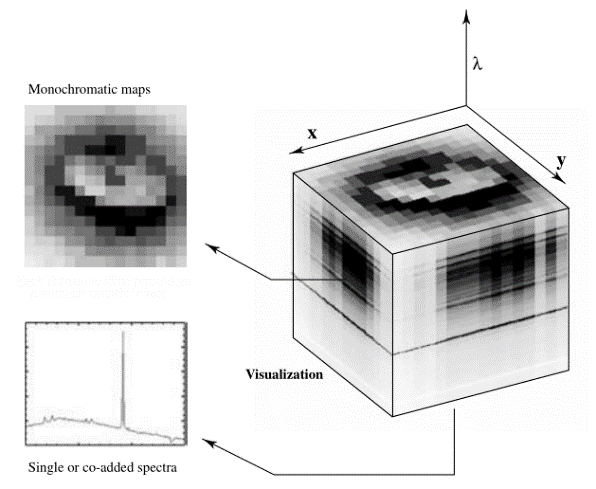
\includegraphics[scale=.80]{imagen1.png}
	\centering	
	\caption{\emph{Representación esquemática de un cubo de datos. (Fuente: 3D Spectroscopy in Astronomy. XVII Canary Island Winter School of Astronomy. Mediavilla, E., Arribas, S., Roth, M.M., Cepa-Nogué, J. \& Sánchez F. 2010. Cambridge University Press)}}
	%\label{imagen1}
\end{figure}

\section{Metodología}
Para este trabajo vamos a utilizar datos de espectroscopia de campo integral. Las observaciones se realizaron con el telescopio de 3.5 m del Observatorio de Calar Alto, con el instrumento PMAS  en modo PPAK, el día 6 de agosto de 2014 (UGC11916). El modo PPAK tiene la configuración denominada ``fibras'', que nos permite obtener mapas con un ancho de campo máximo de 74 x 65 arcsec de forma hexagonal. Esta configuración es especialmente recomendada para la obtención de curvas de rotación galácticas y la observación de galaxias en interacción y regiones HII \textbf{(Barden \& Wade, 1998)}.\\Para este trabajo vamos a usar datos de la línea \hal\ que nos proporcionan información de la posición respecto a la longitud de onda central y del flujo total. Los parámetros estelares que usaremos son la velocidad estelar, la masa luminosa, la intensidad del espectro en su zona central, (concretamente la medida del espectro en una banda de 100 Angstroms, centrada en 5635 Angstroms), la edad pesada en luz, y la extinción estelar. Estos parámetros estelares se han extraído de los cubos de datos utilizando el código \emph{STARLIGHT} \textbf{(Cid Fernandes et al., 2005)}. \emph{STARLIGHT} es un código que compara la distribución espectral de energía observada en los rangos libres de líneas de emisión con un conjunto de librerías de poblaciones estelares a distinta edad y metalicidad, para hallar la distribución de las mismas que ajustan las observaciones con una mejor significación estadística. El código también ajusta las velocidades de desplazamiento de los patrones espectrales observados y la extinción estelar.\\Los datos se nos han proporcionado como tablas o imágenes 2D estandarizados (que denominaremos ``mapas''), por lo que se pueden manejar en software de tratamiento de \emph{FITS} , tipo \emph{DS9} o \emph{QFitsView}.\\Todos los mapas que se muestran en este trabajo tienen la orientación habitual, con el norte hacia arriba y el este a la izquierda, y presentan un ancho de campo de 60 x 60 arcsec.

\subsection{Morfología}
En primer lugar, hemos realizado una caracterización morfológica de la galaxia, para lo que hemos empleado el mapa que nos proporciona la intensidad central del espectro, al que denominaremos ``mapa de señal''. Mediante el trazado de contornos sobre este mapa hemos obtenido diferentes parámetros que nos permiten recabar información sobre la morfología de la galaxia en el continuo. También hemos utilizado imágenes en \hal\ en alta resolución, tomadas con el telescopio de 1,5 m del Observatorio de Sierra Nevada (OSN), el día 3 de agosto de 2013. Estas imágenes tienen mayor resolución y mayor ancho de campo que las del IFU, por lo que nos permiten caracterizar mejor nuestras galaxias. Finalmente, para esta caracterización también nos hemos ayudado de las imágenes del SDSS (Sloan Digital Sky Survey) obtenidas de la base de datos HyperLEDA \textbf{(Makarov et al. 2014)}

\subsection{Análisis de imágenes en alta resolución}
Para determinar la presencia de un anillo, hemos utilizado las imágenes de \hal\ en alta resolución del OSN. Con estas imágenes, hemos buscado y delimitado la presencia de un posible anillo polar para cada nuestra galaxia. En caso de presencia de anillo o de brotes dispersos de $H\alpha$ que pudieran darnos un indicio de la presencia de un anillo, hemos comprobado si se encuentran dentro de los límites de nuestros mapas, que como hemos comentado, tienen un ancho de campo de 60 arcsec, por lo que la distancia máxima del anillo o de los brotes de \hal\ al centro galáctico debe ser inferior a 30 arcsec. Tomando como referencia el mapa de flujo del gas hemos realizado esta comprobación, y en caso afirmativo, hemos delimitado dichas regiones para poder realizar a partir de ellas el resto del estudio.

\subsection{Cinemática}
Para realizar este análisis, en primer lugar, hemos convertido el mapa de posición del gas en mapa de velocidad. Los mapas de posición nos dan la información de la longitud de onda en cada punto. Debido al efecto Doppler, las líneas de emisión se encuentran desplazadas respecto a su valor de referencia en el vacío, por lo que podemos establecer una relación entre ese desplazamiento y su velocidad:
\begin{equation}
v=(\lambda_{0}/\lambda - 1)*c \label{ecuacion_1}
\end{equation}
Siendo $\lambda_{0}$ la longitud de onda observada, $\lambda$ la longitud de onda en el vacío y $c$ la velocidad de la luz.\\De esta forma obtenemos un mapa de velocidad a partir de los mapas de posición, asignando a cada pixel su valor correspondiente de velocidad, en $km/s$. Así, hemos obtenido el mapa de velocidad de \hal. Posteriormente hemos referenciado este mapa al centro de la galaxia, tomando 0 como valor de velocidad en el centro. Para hallar el centro de la galaxia hemos utilizado el mapa de señal y hemos seleccionado el pixel de mayor valor como el centro galáctico. Del mapa de velocidad de \hal\ obtenido anteriormente, hemos restado a cada píxel el valor de la velocidad en el centro galáctico, para de esta manera obtener la velocidad referida al centro de la galaxia en todos los píxeles. Este también lo hemos realizado con el mapa de velocidad estelar, que ya se nos proporcionó en $km/s$. Todo este proceso se ha realizado con el lenguaje de programación \emph{Python}.\\Mediante un análisis de los mapas de la velocidad estelar y de velocidad de \hal\ hemos realizado un estudio de la cinemática de la galaxia. Se ha analizado de manera general los mapas de velocidad, así como el centro galáctico y se han trazado proyecciones para obtener las curvas de rotación tanto del gas como de las estrellas.

\subsection{Poblaciones estelares}
Para el estudio de las poblaciones estelares hemos utilizado los mapas de IFS proporcionados tanto de la edad estelar pesada en luz como de la extinción estelar, analizando la edad global de la galaxia y comparándola con la población estelar del anillo, en los casos en los que el anillo esté presente en nuestros datos. También hemos representado gráficas de distribución de la población estelar tanto de la galaxia como de las zonas en las que hayamos encontrado brotes de emisión en \hal. 

\subsection{Determinación de las propiedades de los anillos}
En caso de haber detectado brotes de HII que nos puedan permitir delimitar un anillo, hemos calculado la velocidad media en esos brotes. Esto lo hemos realizado ayudándonos de la herramienta DS9, tomando las regiones que delimitamos sobre el mapa de flujo y superponiéndolas en los mapas de velocidad referidos al centro galáctico para calcular sus estadísticas. 
En las ocasiones en las que ha sido posible determinar el ángulo de inclinación del anillo con respecto a nuestra línea de visión, se ha corregido la velocidad en función de dicho ángulo. Asumiendo que el anillo se puede inscribir dentro de una elipse, tendríamos la relación:
\begin{equation}
\cos i=(b/a) \label{ecuacion_2}
\end{equation}

Una vez determinado el ángulo de inclinación corregimos la velocidad mediante:
\begin{equation}
v=v_{obs}/\sin i \label{ecuacion_3}
\end{equation}

Conociendo la distancia al centro de la galaxia, podemos definir un radio máximo, y asumiendo que las galaxias se encuentran en equilibrio gravitacional, podemos obtener una estimación sencilla del valor de la masa dinámica aplicando el teorema del virial:

\begin{equation}
M_{D}=(Rv^{2})/G \label{ecuacion_4}
\end{equation}
Donde $M_{D}$ (en $kg$) será la masa dinámica del sistema hasta el radio máximo que hemos definido, $R$ (en $m$) el radio máximo, $v$ (en $m/s$) la velocidad media del anillo o del brote y $G$ (en $m^{3}/kg*s^{2})$ la constante de gravitación Universal. Esta masa dinámica la convertimos en $M_{\odot}$ mediante la relación 1 $M_{\odot} = 1.989 * 10^{30} kg$.
De esta manera, hemos derivado la masa dinámica tanto a partir de las velocidades de rotación del gas como de las estrellas.\\Para calcular la relación entre la masa dinámica y la masa luminosa, podemos determinar la masa luminosa mediante el mapa que nos proporciona información de la masa de cada píxel (en $M_{\odot}$). Sumando el valor de los píxeles dentro del radio delimitado por la galaxia obtenemos el valor de la masa luminosa $M_{L}$.\\Hay que indicar que, en caso de no poder determinar el ángulo de inclinación, los valores obtenidos serán una cota mínima. Incluso con esta corrección, nuestros datos seguirán siendo una cota mínima, pues el radio máximo que hemos definido para derivar la masa dinámica lo hemos delimitado dentro del campo de visión del IFU, y es posible que no sea el radio máximo del anillo.\\ Todos los cálculos y conversión de unidades se han realizado nuevamente a través de \emph{Python}.

\section{Análisis e interpretación de los resultados}
\begin{figure}[H]
	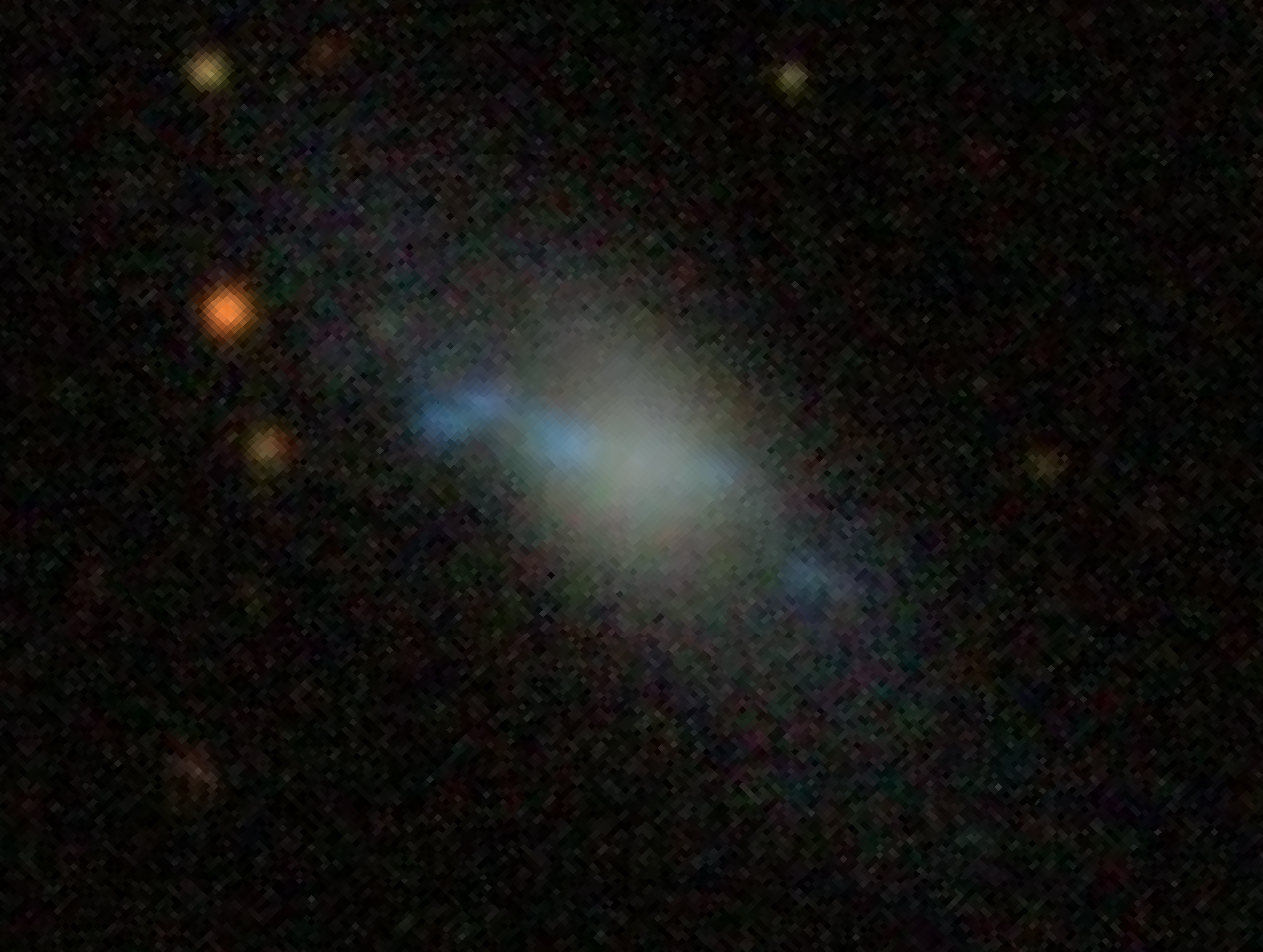
\includegraphics[scale=.20]{imagen2.png}
	\centering	
	\caption{\emph{Imagen de la galaxia UGC11916 (SDSS)}}
	\label{figura 2}
\end{figure}

La galaxia \emph{UGC11916} se encuentra catalogada como una posible \emph{PRG} dentro del catálogo del SDSS \textbf{(Moissev et. al, 2011)}, con el número SPRC-184 (objetos relacionados). Morfológicamente pertenece al tipo \emph{Scd}, una galaxia espiral tardía.

\subsection{Morfología}
\begin{minipage}[b]{0.4\linewidth}
	\begin{figure}[H]
	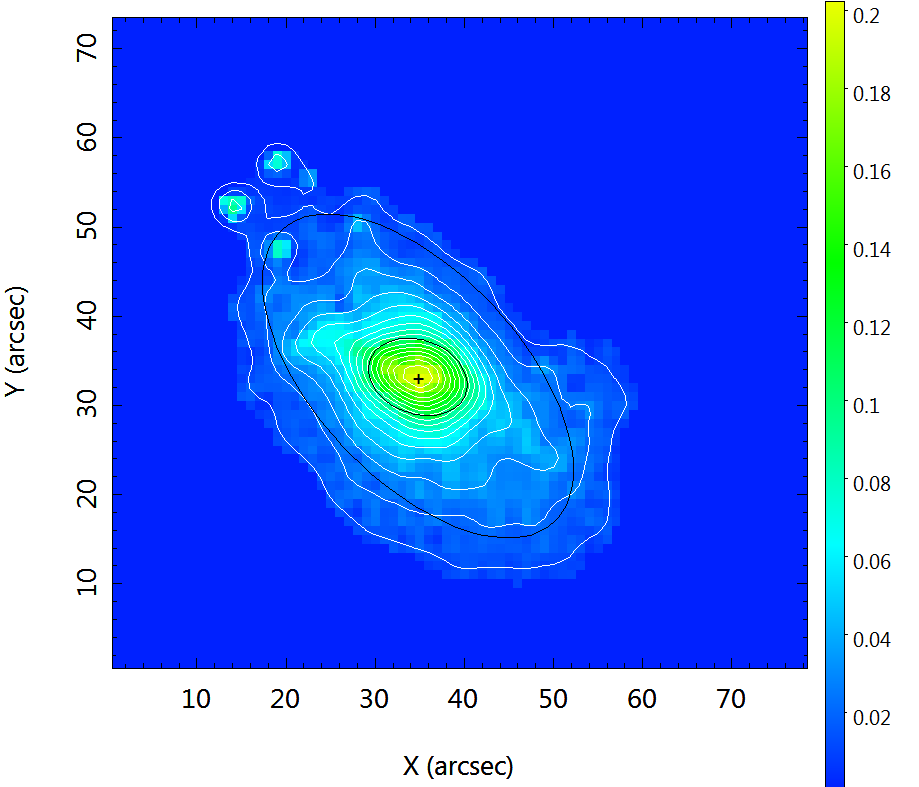
\includegraphics[scale=.20]{imagen3.png}
	\centering	
	\caption{\emph{Mapa de señal de UGC11916}}
	\label{figura 3}
	\end{figure}
\end{minipage} \hfill \begin{minipage}[b]{0.4\linewidth} Los contornos superpuestos sobre el mapa de señal (figura \ref{figura 3}) nos muestran como la zona central de la galaxia, hasta un radio de aproximadamente 7 $arcsec$ (0.6 $kpc$), se inscribe dentro de una elipse con posición angular de unos $70^{\circ}$. En esta zona los contornos son muy regulares, y van distorsionándose según se van alejando del centro, tomando un aspecto irregular en la parte más exterior de la galaxia. Todo el conjunto se puede inscribir en una elipse con una posición angular de $43^{\circ}$.
\end{minipage}\\

\subsection{Análisis de la imagen en alta resolución}
En la imagen del OSN se pueden apreciar dos brotes, siendo el situado al suroeste el que entra dentro de nuestro mapa de flujo de \hal. Para su análisis determinaremos una región circular en la que el flujo es más intenso.

\begin{figure}[H]
	\centering
	\subfigure[ ]{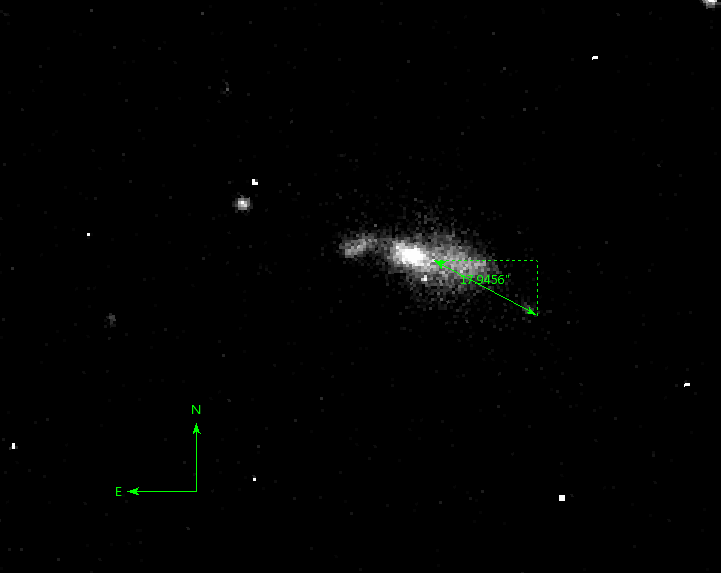
\includegraphics[scale=.28]{imagen4.png}}
	\subfigure[ ]{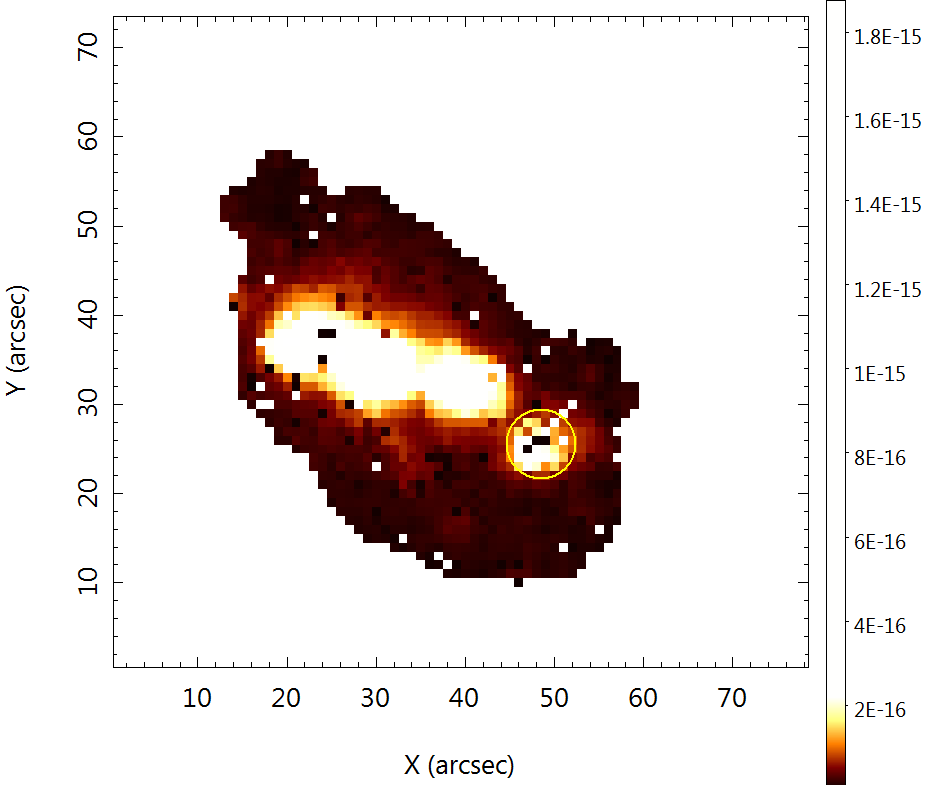
\includegraphics[scale=.20]{imagen5.png}}
	\caption{\emph{a) Imagen $H\alpha$ de la galaxia UGC11916 (SDSS), b) Mapa de flujo}}
	\label{figura 4}
\end{figure} 

\subsection{Cinemática}
En el mapa de velocidad de \hal\ (figura \ref{figura 5}a) podemos ver como parece que el gas está rotando en la dirección del eje mayor de la galaxia, la parte noreste se aleja de nosotros mientras que la parte suroeste se acerca. La diferencia de velocidades es por lo general muy pequeña en toda la galaxia. El mapa de velocidad estelar nos muestra un patrón muy irregular (figura \ref{figura 5}b). Es difícil distinguir una rotación evidente.
\begin{figure}[H]
	\centering
	\subfigure[ ]{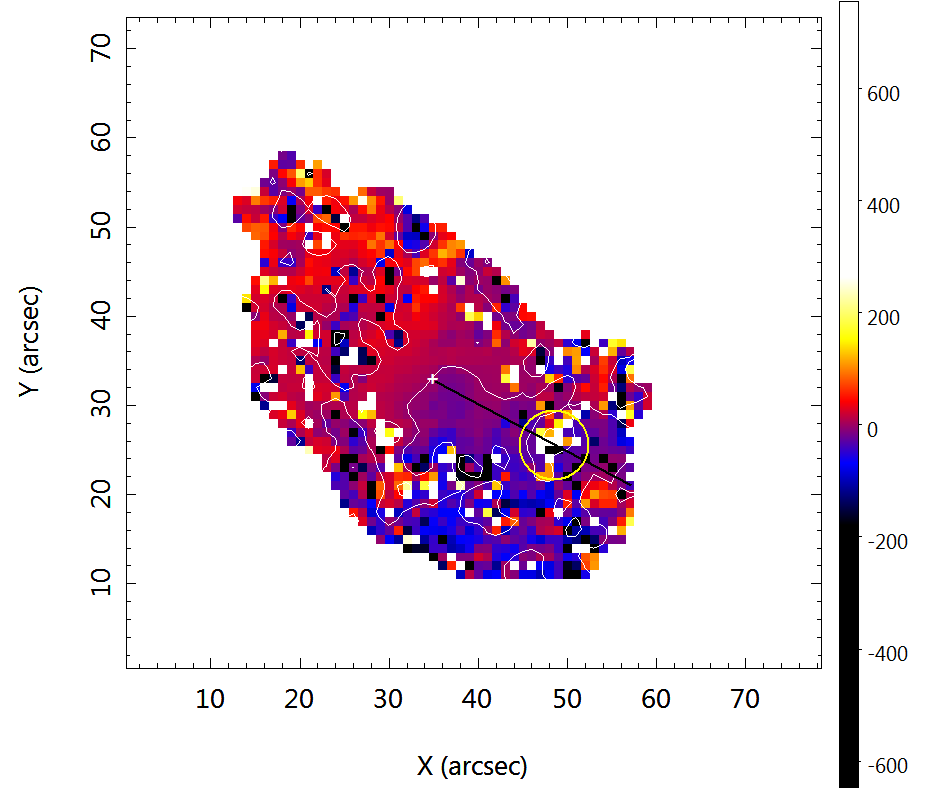
\includegraphics[scale=.20]{imagen6.png}}
	\subfigure[ ]{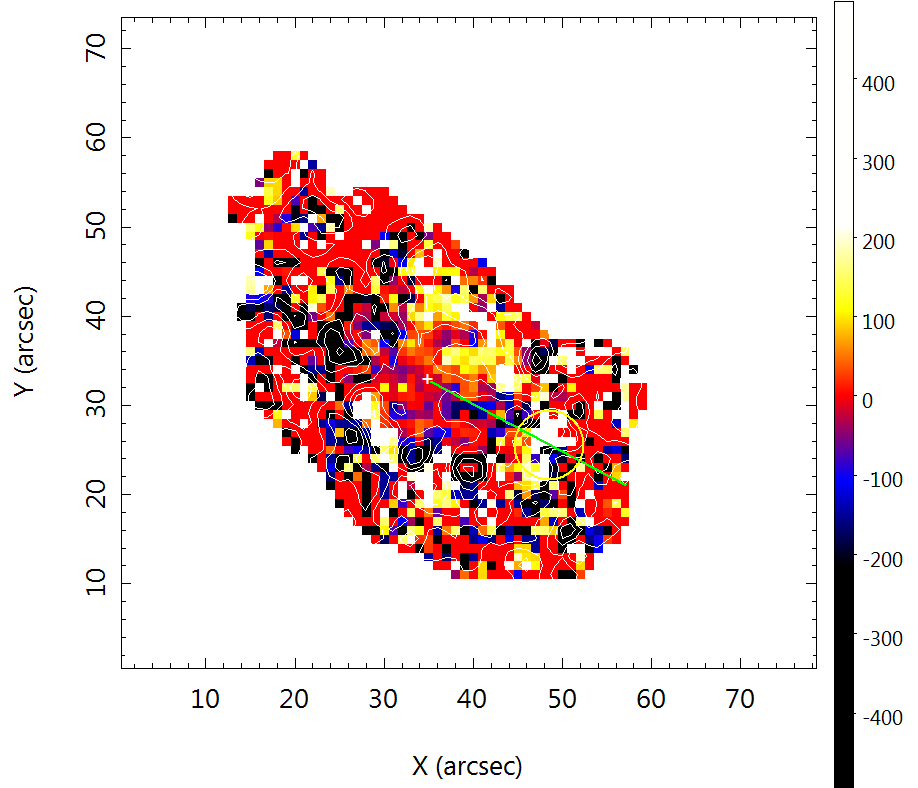
\includegraphics[scale=.20]{imagen7.png}}
	\caption{\emph{Mapas de velocidad del gas (a) y estelar (b)}}
	\label{figura 5}
\end{figure} 
A pesar de la irregularidad del mapa de velocidad estelar, las proyecciones sobre ambos mapas trazadas desde el centro galáctico pasando por la región seleccionada para el análisis nos muestran una gran similitud (figura \ref{figura 6})\footnote{El centro galáctico se encuentra en la coordenada (35,32)}, en la que en ambos casos se aprecia como la velocidad es en ambos casos negativa y relativamente constante, especialmente en el caso del gas. Al llegar a la zona donde comienza nuestra región aumenta considerablemente, llegando en ambos casos a superar los 400 $km/s$, volviendo a descender de un modo brusco al salir de la región y adquiriendo valores próximos a los que había en un principio. Este cambio brusco nos hace pensar que la región analizada forma un sistema cinemático independiente del resto de la galaxia, esto es, forma parte de un anillo. Aun así, no podemos asegurarlo con certeza, puesto que en las medidas de velocidades podemos encontrar datos que nos sugieran relaciones espurias, como podría ser este caso.
\begin{figure}[H]
	\centering
	\subfigure[ ]{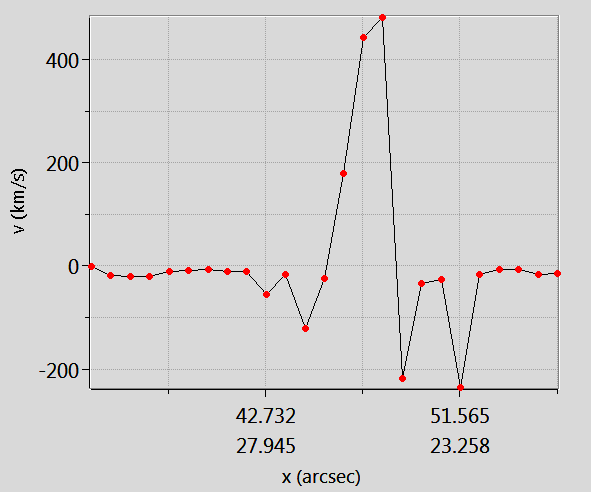
\includegraphics[scale=.35]{imagen8.png}}
	\subfigure[ ]{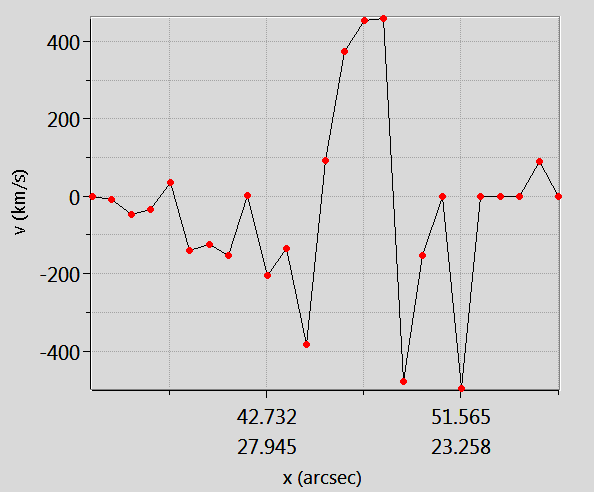
\includegraphics[scale=.35]{imagen9.png}}
	\caption{\emph{Curvas de velocidad del gas (a) y estelar (b)}}
	\label{figura 6}
\end{figure} 

\subsection{Poblaciones estelares}
Al analizar el mapa de población estelar (figura \ref{figura 7}a), podemos observar como la zona central de la galaxia es la zona donde la población es mayoritariamente del tipo II, con edades entre 1 y 5 $Ga$. También se aprecia como en la parte más exterior sureste forma un brazo en el que la población no supera los 100 $Ma$, algo característico en los brazos de las galaxias espirales como ya hemos indicado. También podemos observar que en la zona donde se encuentra nuestra región, y de manera casi perpendicular al eje mayor de la galaxia, podemos encontrar también una gran acumulación de población I, algo que refuerza nuestra idea de que la región analizada forma parte de un anillo polar.\\Podemos observar que la correlación entre la extinción estelar (figura \ref{figura 7}b) y las poblaciones es evidente al comparar ambos mapas, comprobando que en las zonas donde la población es más joven la extinción es mayor, debido a que en estas zonas la cantidad de polvo es mucho mayor.
\begin{figure}[H]
	\centering
	\subfigure[ ]{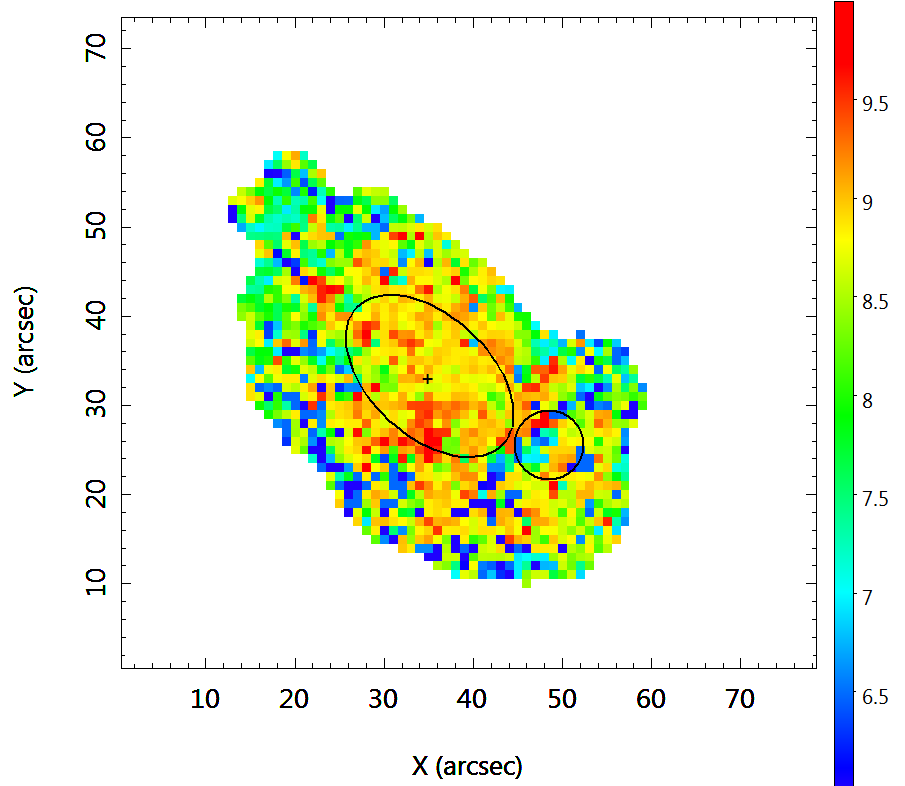
\includegraphics[scale=.20]{imagen10.png}}
	\subfigure[ ]{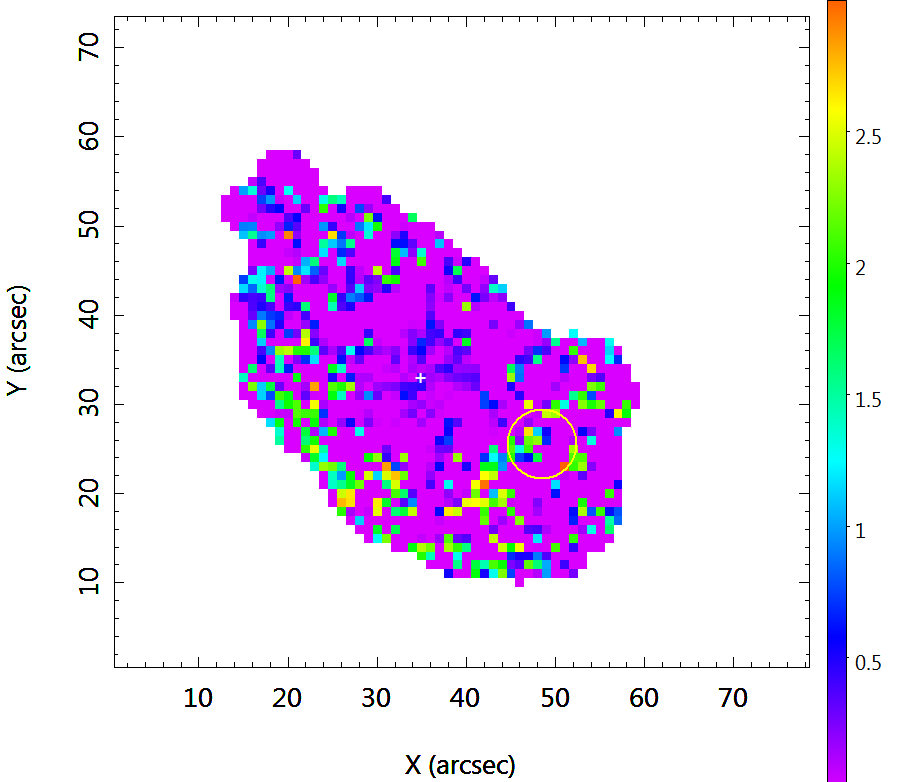
\includegraphics[scale=.20]{imagen11.png}}
	\caption{\emph{Mapa de población estelar pesada en luz (a) y mapa de extinción (b)}}
	\label{figura 7}
\end{figure} 
En la figura \ref{figura 8}a podemos observar los gráficos de distribución de las edades de las poblaciones estelares. Vemos en que la población de esta galaxia es muy joven, con una gran cantidad de población I. En la figura \ref{figura 8}b tenemos la distribución de las edades en la región estudiada mientras que en la figura \ref{figura 8}c tenemos la distribución de las edades en la zona central definida por la elipse que se muestra en la figura \ref{figura 7}a.
\begin{figure}[H]
	\centering
	\subfigure[ ]{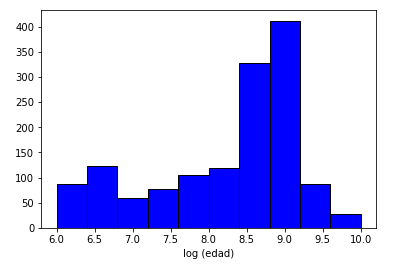
\includegraphics[scale=.50]{imagen12.png}}
	\subfigure[ ]{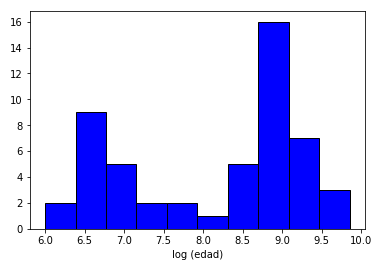
\includegraphics[scale=.50]{imagen13.png}}
	\subfigure[ ]{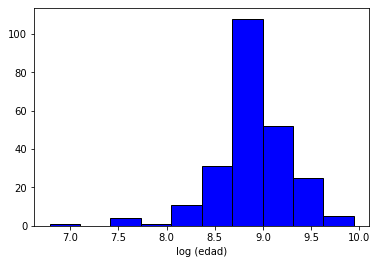
\includegraphics[scale=.50]{imagen14.png}}
	\caption{\emph{Distribución de la población estelar de la galaxia (a), de la región seleccionada (b) y de la región central (c)}}
	\label{figura 8}
\end{figure} 

\subsection{Determinación de las propiedades del anillo}
En nuestra región seleccionada, obtenemos mediante la ecuación \ref{ecuacion_3} que el gas tiene una velocidad media referida al centro galáctico $vH\alpha = 8.84425\ km/s$, mientras que la distancia de esa región al centro de la galaxia, situado en la coordenada (35, 32), es de $16.0137\ arcsec$ ($1.42\ kpc$). Si aplicamos la ecuación \ref{ecuacion_4}, la masa dinámica obtenida a partir de las velocidades del gas es de $M_{D} = 2.584*10^{7}\ M_{\odot}$. El valor de la masa luminosa de la galaxia obtenida de nuestro mapa de IFS es de $3.2347*10^{8}\ M_{\odot}$, obteniendo una relación $M_{D} / M_{L}$ de 0.08.
En esa misma región hemos analizado el mapa de velocidad estelar. La velocidad media referida al centro en este caso es de $vest = 64.6225\ km/s$, con lo que el valor de la masa dinámica obtenida a partir de las velocidades estelares es de $MD = 1.3795*10^{9}\ M_{\odot}$, y la relación $M_{D} / M_{L}$ en este caso es 4.26. 
Como ya hemos indicado, estos valores representan una cota mínima, al no poder estimar el ángulo de inclinación del posible anillo. Comprobamos que, a pesar de esto, la masa dinámica derivada a partir de las velocidades estelares es mayor que la masa luminosa. A pesar de encontrarse dentro de la relación de \emph{Taylor et al (2010)}, la masa luminosa de nuestra galaxia es menor que la masa luminosa de la muestra de Taylor.\\

\begin{table}[H]
\centering
\begin{tabular}{cccc} \toprule
%\hline
Datos & $v(km/s)$ & $MD(M_{\odot})$ & $M_{D} / M_{L}$\\ \midrule
%\hline
$H\alpha$ & $8.84426$ & $2.584*10^{7}$ & $0.08$\\
%\hline
Estelar & $64.225$ & $1.3795*10^{9}$ & $4.26$\\ \bottomrule
\end{tabular}
\caption{Valores obtenidos para la galaxia UGC11916}
\label{Tabla_1}
\end{table}

\section{Conclusiones}

Hemos analizado los datos de la galaxia UGC11916, analizando un brote de HII y hemos decidido que forma parte de un anillo polar al estudiar las curvas de velocidad tanto del gas como de las estrellas. El estudio de las poblaciones estelares ha reforzado nuestra decisión de incluir esa región en un anillo.
Hemos podido comparar la masa dinámica con la masa luminosa de la galaxia, obteniendo que la masa dinámica derivada a partir de las velocidades estelares es mayor que la masa luminosa, en una relación que coincide con la encontrada por Taylor y sus colaboradores \emph{(Taylor et al. 2010)} para las galaxias con redshift z ~ 0, como es el caso de la nuestra, si nuestra galaxia presenta una masa luminosa menor que la masa de la muestra empleada por Taylor para su estudio. Los valores de la masa dinámica derivada a partir de las velocidades del gas no son aceptables incluso tratándose de valores de cota mínima, lo que nos confirma que nuestra estimación de velocidades y del radio máximo no han sido correctas. Con los resultados obtenidos podemos concluir que la diferencia entre la masa dinámica y la masa luminosa es debida a la presencia de materia no bariónica, es decir, debido a la componente de materia oscura en las galaxias \emph{(Padmanabhan et al. 2003)}. En el cuadro \ref{Tabla_2} se muestra un resumen de los datos obtenidos. La tercera columna, indica si en nuestro trabajo hemos podido determinar la presencia de anillo en la galaxia estudiada.

\begin{table}[H]
\centering
\scalebox{0.8}{
\begin{tabular}{cccccccc} \toprule
%\hline
{} & {} & {} & $M_{L}$ &$M_{D}(H\alpha)$ & $M_{D}/M_{L}$ & $M_{D} (est)$ & $M_{D}/M_{L}$\\
Galaxia & Tipo & Anillo & $(M_{\odot}$) & $(M_{\odot}$) & $H\alpha$ & $M_{\odot}$ & $est$\\
\midrule
%\hline
$UGC11916$ & $Scd$ & Sí & $3.2347*10^{8}$ & $2.584*10^{7}$ & $0.08$ & $13.3795*10^{9}$ & $4.26$\\ \bottomrule
\end{tabular}}
\caption{Valores obtenidos para la galaxia UGC11916}
\label{Tabla_2}
\end{table}


\bibliographystyle{unsrt}
\bibliography{astro}

\end{document}
